\documentclass[12pt,reqno]{amsart}

\usepackage{amsthm,amsmath,amssymb}
\usepackage{mathtools}
\usepackage{xcolor}
\usepackage{graphicx,wrapfig}
\usepackage[T1]{fontenc}
\usepackage{courier}
\usepackage{hyperref}
\hypersetup{
    hidelinks=true
}
\usepackage{array}
\usepackage{multirow}
\usepackage{listings}
\lstset{basicstyle=\ttfamily\footnotesize, columns=fullflexible, language=C, morekeywords={omp,task,private,pragma,parallel,reduction,single,nowait,num_threads}, numbers=left}
\newcommand{\code}[1]{\texttt{#1}}
\newcommand\MyBox[2]{
  \fbox{\lower0.75cm
    \vbox to 1.7cm{\vfil
      \hbox to 1.7cm{\hfil\parbox{1.4cm}{#1\\#2}\hfil}
      \vfil}%
  }%
}
\graphicspath{{./}}

\begin{document}

\begin{center}
\large\textbf{Assignment 2 \\ COMP529 Fall 2019 - Parallel Programming} \\
\normalsize\textbf{Erhan Tezcan 0070881 \\ 26.04.2020} \\
\end{center}

As per request, this first paragraph will present my results. The sections that follow the end of this paragraph will be about my design and implementation as well as interpretation of the performance findings in detail. I have 4 versions of the parallel code, 3 of them were the ones requested in the assignment and $4^{\text{th}}$ one is the best performing one with different optimizations. We discuss the performance results in depth at the last section. Our best performing version was version 4, where we used shared memory reduction. For block size $32\times32$ and $16\times16$, best combination of optimizations in version 4 were to use shared memory sum reduction, global access for both compute kernels and pinned memory. For block size $8\times8$ however, interestingly, best combination of optimizations were to use shared memory sum reduction, global access for compute 1 kernel, shared memory with direction-wise halo checks for compute 2 kernel and no pinned memory. Below is a graph showing the speedups for all versions and block sizes (figure \ref{fig:speedallintro}):
\begin{figure}[h]
\centering
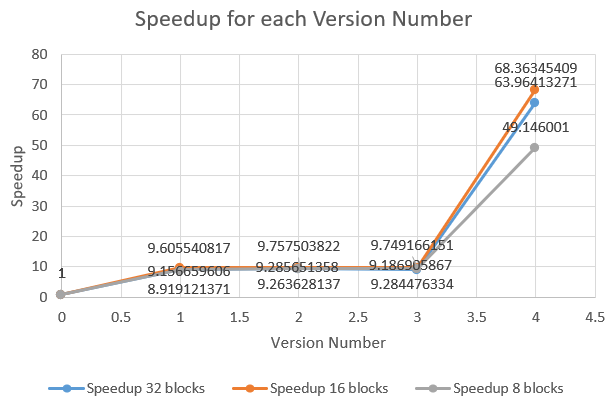
\includegraphics[width=0.92\linewidth]{speedall.png}
\caption{Speedups for each version. Version 0 is serial. The rest are parallel. Version 1 is using global access only. Version 2 is using registers for data re-use. Version 3 uses shared memory on compute 2 kernel. Version 4 is a combination of optimizations and is the best version.}
\label{fig:speedallintro}
\end{figure}
To state explicitly, for block size $16\times16$ my GFLOP values are:
\begin{itemize}
	\item \textbf{Version 0 (Serial):} 1.043445
	\item \textbf{Version 1 (Naive Parallel):} 10.02285
	\item \textbf{Version 2 (Registers):} 10.181423
	\item \textbf{Version 3 (Shared Memory in Compute 2 Kernel):} 10.172723
	\item \textbf{Version 4 (Best Version):} 71.333534
\end{itemize}
We will discuss these results at the end of this report. We will be interpreting why we do not see performance improvements between some versions and why block size matters. We will also explain how we chose the best version and how we decided which optimizations to use. 
All codes in this report are compiled with \code{-O3} option, and they were ran using a \code{Tesla K20M} gpu that is found in KUACC. The target image was \code{coffee.pgm} for all results and we had 100 iterations, by passing \code{-iter 100} command line option.

\section{Objective}

We are asked to implement ``Accelerated Image Denoising'' on CUDA. We are given the serial code for this and in that code the parallelizable parts are specified rather clearly. We will not go into details of the algorithm in this report, but rather how the memory accesses are and how we can obtain performance from these computations. The algorithm in general has 3 parts: reduction, computation 1 and computation 2. However, we will actually talk about 4 parts here:
\begin{itemize}
	\item Reduction
	\item Statistics
	\item Computation 1
	\item Computation 2
\end{itemize}
Each part depends on the one above, thus requires some form of synchronization in between. There is also a synchronization between Computation 2 and Reduction, such that Reduction may not start before Computation 2 ends. Statistics depend on Reduction too, because statistics use the result of that sum reduction.

First, we will look at our implementations, and then we will see the performance comparions and draw conclusions from those.

\section{Design \& Implementation}

In my implementation, I have 4 versions, so that is one more than what was asked:
\begin{enumerate}
	\item Naive Parallel \\
	Global memory accesses are used only.
	\item Registers \\
	Multiple global memory accesses on the same location are first stored in register and then accessed over that register.
	\item Shared Memory \\
	Only on Compute 2 kernel we use shared memory.
	\item Shared Memory and Reduction \\
	We use shared memory on all kernels, especially on sum reduce.
\end{enumerate}

Before we start the versions, we have to look at our grid and block dimensions. For a block, I have used $32\times32$ threads, so a total of 1024 per block; in other words, $block_x = 32, block_y = 32$. For the grid, we used the dimensions below:
$$
grid_x = \left\lceil \frac{width}{block_x}\right\rceil
$$
$$
grid_y = \left\lceil \frac{height}{block_y}\right\rceil
$$
where $width$ and $height$ are the dimensions of the image, respectively. This way, we effectively divide the image on to blocks on GPU, with equally sized granularities.

We utilize CUDA streams on all our versions. At the host side, the compute part is done like this:
\begin{figure}[h]
\centering
\begin{lstlisting}
for each iteration do
    issue memset 0 to reset sum variables
    issue reduction kernel with grid and block parameters
    issue statistics kernel on a single block with single thread
    issue compute 1 kernel with grid and block parameters
    issue compute 2 kernel with grid and block parameters 
end for
\end{lstlisting}
\caption{Stream and Kernels}
\label{fig:hostloop}
\end{figure}

We don't use asynchronous \code{memcpy} operations because that would change our time calculations. Using stream in this way ensures the in-between kernel synchronization. Another benefit of this is that, we effectively issue all kernels and be done with the loop at host side thanks to stream mechanism. This gives us a slight advantage compared to calling \code{cudaDeviceSynchronize} after every kernel.

\subsection{Version 1 - Naive Parallel}
This version is more of a copy-paste of the serial version than coding. However, we have to write some extra code for the device allocations and data transfers. We use global memory accesses only, so our kernels are very much like their counterparts in the serial version. 

\subsubsection{Reduction} For the sum reduction, we have this kernel below:
\begin{figure}[h]
\centering
\begin{lstlisting}
__global__ void reduction_kernel(unsigned char* image, int width, int height, 
            int n_pixels, float* sum, float* sum2) { 
  int j = blockIdx.x * blockDim.x + threadIdx.x;
  int i = blockIdx.y * blockDim.y + threadIdx.y;
  if (j >= 0 && j < width && i >= 0 && i < height) {
    long p = (i * width + j);
    float tmp = image[p];
    atomicAdd(&sum[0], tmp);
    atomicAdd(&sum2[0], tmp * tmp); 
  }	
}
\end{lstlisting}
\label{fig:redkern}
\caption{Reduction Kernel with global access only}
\end{figure}

We see that the additions on \code{sum} and \code{sum2} are just as if they are serial, because only one thread can edit them at a time: this is thanks to the \code{atomicAdd} device function provided by CUDA. We also see that the sum variables are actually pointers. They point to a single float sized array on the device, thus they are actually scalars; it's just that instead of writing \code{sum} we write \code{sum[0]} to access them. This kernel is launched with the $grid$ and $block$ parameters we discussed above.

\subsubsection{Statistics} Then comes the statistics kernel, seen in figure \ref{fig:statsk}. This is the kernel that calculates standart deviation based on both sum values. Unlike other kernels, this one is launched by a single block, with a single thread in it.

The reason we split the reduction and statistics part like this is because this kernel depends on the completion of sum reduction. By using streams, and isuing these two kernels in order, we obtain that synchronization required to match the completion of sum reduction. 

\begin{figure}[!h]
\centering
\begin{lstlisting}
__global__ void statistics_kernel(float* sum, int n_pixels, float* sum2, 
            float* std_dev) { 
  float mean = sum[0] / n_pixels;
  float variance = (sum2[0] / n_pixels) - mean * mean;
  std_dev[0] = variance / (mean * mean);
}
\end{lstlisting}
\caption{Statistics kernel.}
\label{fig:statsk}
\end{figure}

\subsubsection{Compute 1} 

This kernel is just like serial version, we only do some indexing instead of the for loop. This is also launched with the $grid$ and $block$ parameters we discussed above. Figure \ref{fig:c1kernel_reg} shows the code.
\begin{figure}[!h]
\centering
\begin{lstlisting}
__global__ void compute1_kernel(unsigned char* image, int width, int height,
            int n_pixels, float* std_dev, float* north_deriv, float* south_deriv, 
            float* west_deriv, float* east_deriv, float* diff_coef) {
  int j = blockIdx.x * blockDim.x + threadIdx.x; 
  int i = blockIdx.y * blockDim.y + threadIdx.y;
  if (j > 0 && j < width - 1 && i > 0 && i < height - 1) {
    float gradient_square, num, den, std_dev2, laplacian;
    long k = i * width + j;	// position of current element
    north_deriv[k] = image[k - width] - image[k];
    south_deriv[k] = image[k + width] - image[k];
    west_deriv[k] = image[k - 1] - image[k];
    east_deriv[k] = image[k + 1] - image[k];
    gradient_square =(north_deriv[k]*north_deriv[k]+south_deriv[k]*south_deriv[k]
            + west_deriv[k]*west_deriv[k]+east_deriv[k]*east_deriv[k]) 
            / (image[k] * image[k]);
    laplacian=(north_deriv[k]+south_deriv[k]+west_deriv[k]+east_deriv[k])/image[k];
    num = (0.5 * gradient_square) - ((1.0 / 16.0) * (laplacian * laplacian)); 
    den = 1 + (.25 * laplacian);
    std_dev2 = num / (den * den); 
    den = (std_dev2 - std_dev[0]) / (std_dev[0] * (1 + std_dev[0]));
    diff_coef[k] = 1.0 / (1.0 + den);
    if (diff_coef[k] < 0) {
        diff_coef[k] = 0;
    } else if (diff_coef[k] > 1) {
        diff_coef[k] = 1;
    }
  }	
}
\end{lstlisting}
\caption{Compute 1 Kernel with global access}
\label{fig:c1kernel_reg}
\end{figure}

\clearpage

\subsubsection{Compute 2} 

Just like the previous kernel, this is same as serial version, and is again launched with $grid$ and $block$ parameters. Figure \ref{fig:c2kernel_reg} shows the code.

\begin{figure}[h]
\centering
\begin{lstlisting}
__global__ void compute2_kernel(float* diff_coef, int width, int height, 
            float lambda, float* north_deriv, float* south_deriv, 
            float* west_deriv, float* east_deriv, unsigned char* image) {
  int j = blockIdx.x * blockDim.x + threadIdx.x;
  int i = blockIdx.y * blockDim.y + threadIdx.y;
  if (j > 0 && j < width - 1 && i > 0 && i < height - 1) {
    float diff_coef_north,diff_coef_south,diff_coef_east,diff_coef_west,divergence;
    long k = i * width + j; 
    diff_coef_north = diff_coef[k];	
    diff_coef_south = diff_coef[k + width];	
    diff_coef_west = diff_coef[k];	
    diff_coef_east = diff_coef[k + 1];			
    divergence = diff_coef_north*north_deriv[k]+diff_coef_south*south_deriv[k]+
        diff_coef_west*west_deriv[k]+diff_coef_east*east_deriv[k];
    image[k] = image[k] + 0.25 * lambda * divergence; 
  }
}
\end{lstlisting}
\caption{Compute 2 Kernel with global access}
\label{fig:c2kernel_reg}
\end{figure}

\subsection{Version 2 - Registers}
This version is very similar to the version before, with one main difference: \textit{if a global memory is accessed multiple times, we store it on a register and use that register for all accesses.}

This way, instead of global memory, we will access the registers, which have the fastest access by the threads. This will give us a slightly better performance compared to global access. We do not want to populate this section with the same codes again, so we will move on to the next section where we willl do shared memory for Compute 2 kernel.

\subsection{Version 3 - Shared Memory}
In this version, we will focus on Compute 2 Kernel only, as it is the only difference between the previous version.
\begin{figure}[h]
\centering
\begin{lstlisting}
__global__ void compute2_kernel(float* diff_coef, int width, int height, 
            float lambda, float* north_deriv, float* south_deriv, 
            float* west_deriv, float* east_deriv, unsigned char* image) {
  unsigned int col = blockIdx.x * blockDim.x + threadIdx.x;
  unsigned int row = blockIdx.y * blockDim.y + threadIdx.y;
  __shared__ unsigned char sdata[DIM_THREAD_BLOCK_Y][DIM_THREAD_BLOCK_X+1];
  float diff_coef_k;
  int tx = threadIdx.x;
  int ty = threadIdx.y; 
  long k;
  if (col < width && row < height) {
    k = row * width + col; 
    diff_coef_k = diff_coef[k];
    sdata[ty][tx] = diff_coef_k;
  }
  __syncthreads();	
  if (col > 0 && col < width - 1 && row > 0 && row < height - 1) {
    float divergence;
    if (tx == blockDim.x - 1 && ty == blockDim.y - 1) {
        divergence =diff_coef_k*north_deriv[k]+diff_coef[k + width]*south_deriv[k] 
        + diff_coef_k * west_deriv[k] + diff_coef[k + 1] * east_deriv[k];
    } else if (tx == blockDim.x - 1) {
        divergence =diff_coef_k*north_deriv[k]+sdata[ty+1][tx]*south_deriv[k] 
        + diff_coef_k * west_deriv[k] + diff_coef[k + 1] * east_deriv[k];
    } else if (ty == blockDim.y - 1) {			
        divergence =diff_coef_k*north_deriv[k]+diff_coef[k + width]*south_deriv[k] 
        + diff_coef_k * west_deriv[k] + sdata[ty][tx+1] * east_deriv[k];
    } else {
        divergence =diff_coef_k*north_deriv[k]+sdata[ty+1][tx]*south_deriv[k] 
        + diff_coef_k * west_deriv[k] + sdata[ty][tx+1] * east_deriv[k];
    }
    image[k] = image[k] + 0.25 * lambda * divergence;
  }
}
\end{lstlisting}
\caption{Compute 2 Kernel with Shared Memory}
\label{fig:c2kernel_shared}
\end{figure}

In the algorithm (seen on figure \ref{fig:c2kernel_shared}), only south and east neighbor is used. However, we will explain our shared memory implementation as if it uses all 4 directions as neighbor. This way, same explanation will apply for shared memory implementation of Compute 1 kernel. In this shared memory implementation, each thread in the block (as long as they are able to index the image) load the pixel to the shared memory. Then, depending on the position of the pixel on the image, we use shared memory or do a global access. Global access happens on the ``halo'' region. We will show this in a better way with a figure. See figure \ref{fig:shmem1} (a), there, the green box is shared memory. It is actually the block of threads loading one pixel each from the image to the shared memory. The gray rectangles are halo regions, they are not loaded to shared memory but they are used by this kernel. A side-note, we have another implementation which we will discuss later that loads the halo to the shared memory too. The other colorful boxes are single threads: blue box shows a thread that loads 3 values from shared memory and one from the global memory, orange box shows a thread that loads 2 values from shared memory and 2 from the global memory. Yellow loads everything from shared memory. On figure \ref{fig:shmem1} (b) we want to show that this algorithm is robust against image borders too. The first block corresponds to upper left of the image. All threads participate in image loading, however for the compute part there is a margin of 1 pixel. Therefore, only light green threads work, and the dark greens do not. However, since dark green pixels loaded the pixels, the light green threads are able to use them.

\begin{figure}[h]
\centering
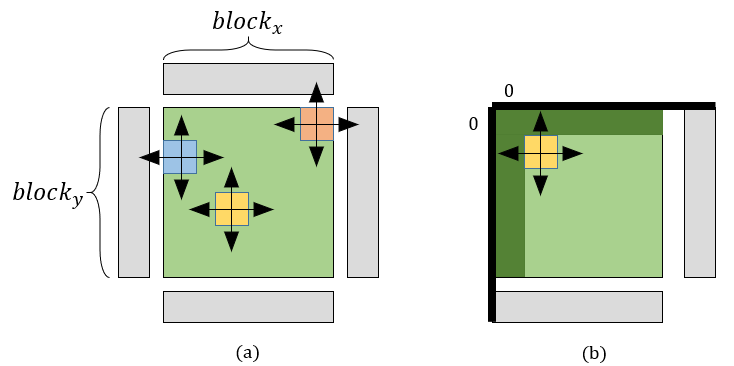
\includegraphics[width=0.9\linewidth]{shmemaccessv1.png}
\caption{Shared Memory with direction-wise halo checks. (version 1)}
\label{fig:shmem1}
\end{figure}

The way we check the boundary condition to whether do a global access or use shared memory is done for each direction separately here. For example, if my column is not 0 and I am the leftmost side of the block, I have to do a global access. There are other versions of this implementation, but we will discuss them later.

\subsection{Version 4 - Best Performing version}
In this version, we have implemented shared memory and sum reduction all together. Then we have tried all combinations and chose the best performing one. Our choices were like this:
\begin{itemize}
	\item Reduction, 2 options:
	\begin{itemize}
		\item Do shared memory sum reduction
		\item Do global access only
	\end{itemize}
	\item Statistics, no option. This is implemented as it was in version 2 (see figure \ref{fig:statsk}).
	\item Compute 1 Kernel, 4 options:
	\begin{itemize}
		\item Shared Memory with Direction-wise halo checks
		\item Shared Memory with Index-wise halo checks
		\item Fully Shared Memory with no halo checks
		\item Global access only
	\end{itemize}
	\item Compute 2 Kernel, 4 options:
	\begin{itemize}
		\item Shared Memory with Direction-wise halo checks
		\item Shared Memory with Index-wise halo checks
		\item Fully Shared Memory with no halo checks
		\item Global access only
	\end{itemize}
\end{itemize}

Compute 1 Kernel and Compute 2 Kernel have almost the same memory access pattern, therefore their shared memory implementations are also the same. In the end we have decided that the best version (in general) is:
\begin{itemize}
	\item Reduction with shared memory sum reduction
	\item Statistics
	\item Compute 1 Kernel with global access only
	\item Compute 2 Kernel with global access only
\end{itemize}
Only exception to this was when we have used block size $8\times8$. Now we will step by step explain our optimizations. First we will look at reduction.

\subsubsection{Sum Reduction}
In our implementation, we have 2 reduction kernels.

\begin{figure}[h]
\centering
\begin{lstlisting}
__global__ void reduction_kernel_1(unsigned char* image, int width, int height, 
            int n_pixels, float* reduarr_sum1, float* reduarr_sum2) { 
  unsigned int j = blockIdx.x * blockDim.x + threadIdx.x;
  unsigned int i = blockIdx.y * blockDim.y + threadIdx.y;
  __shared__ unsigned char sdata_1[DIM_THREAD_BLOCK_X * DIM_THREAD_BLOCK_Y];
  __shared__ unsigned char sdata_2[DIM_THREAD_BLOCK_X * DIM_THREAD_BLOCK_Y];
  if (j < width && i < height) {
    int k = i * width + j;
    int tid = threadIdx.y * blockDim.x + threadIdx.x; 
    float image_k = image[k]; 
    sdata_1[tid] = image_k;
    sdata_2[tid] = image_k * image_k; 
    __syncthreads();
    for (unsigned int s=(DIM_THREAD_BLOCK_X*DIM_THREAD_BLOCK_Y)/2;s>0;s>>=1) {
      if (tid < s) {
        sdata_1[tid] += sdata_1[tid + s];
        sdata_2[tid] += sdata_2[tid + s] * sdata_2[tid + s]; 
      }
    __syncthreads();
    }
    if (tid == 0) {
      reduarr_sum1[blockIdx.y * blockDim.x + blockIdx.x] = sdata_1[0];
      reduarr_sum2[blockIdx.y * blockDim.x + blockIdx.x] = sdata_2[0];
    }		
  }		
}
\end{lstlisting}
\caption{Reduction Kernel with Shared Memory Sum Reduction, part 1. Launched with $grid$ and $block$ parameters.}
\label{fig:reduc_1}

\end{figure}

On figure \ref{fig:reduc_1} we see how the first part of the reduction takes place. We said that the image has dimensions $width$ and $height$, and our grid dimension is $grid_x \times grid_y$ as well as the block dimension $block_x \times block_y$. Each block here will obtain one result from this reduction, so from the $width \times height$ values we reduce to $grid_x \times grid_y$ values. Note that the reduction is simultaenously happening for both sum variables. The results are written to arrays \code{reduarr\_sum1} and \code{reduarr\_sum2}. Then the next reduction takes place.

\begin{figure}[h]
\centering
\begin{lstlisting}
__global__ void reduction_kernel_2(float* reduarr_sum1, float* reduarr_sum2, 
			int n, float* sums) {
  unsigned int i = blockIdx.x * blockDim.x * 2 + threadIdx.x;
  __shared__ unsigned char sdata_1[DIM_THREAD_BLOCK_X * DIM_THREAD_BLOCK_Y];
  __shared__ unsigned char sdata_2[DIM_THREAD_BLOCK_X * DIM_THREAD_BLOCK_Y]; 
  if (i <= n) {
	int tid = threadIdx.x; 
	sdata_1[tid] = reduarr_sum1[i] + reduarr_sum1[i + blockDim.x];
	sdata_2[tid] = reduarr_sum2[i] + reduarr_sum2[i + blockDim.x]; 
	__syncthreads();
	for (unsigned int s = blockDim.x/2; s>0; s>>=1) {
	  if (tid < s) { 
		sdata_1[tid] += sdata_1[tid + s]; 
		sdata_2[tid] += sdata_2[tid + s];
	  }
	  __syncthreads();
	}
	if (tid == 0) {
	  atomicAdd(&sums[0], sdata_1[0]);
	  atomicAdd(&sums[1], sdata_2[0]);
	}
  }		
}
\end{lstlisting}
\caption{Reduction Kernel with Shared Memory Sum Reduction, part 2. Launched with $newgrid$ and $newblock$ parameters.}
\label{fig:reduc_2}
\end{figure}
 
 After reducing to $grid_x \times grid_y$, we reduce it again. This time we launch a different grid block configuration. Now, our block is 1D insteadof 2D, but still the same size (1024 threads). The grid dimension is also 1D, and is calculated like this:
 $$
 newgrid_x = \left\lceil \frac{grid_x \times grid_y}{block_x \times block_y}\right\rceil
 $$
 $$
 newblock_x = block_x \times block_y
 $$
 We launch the kernel given on figure \ref{fig:reduc_2} with the $newgrid$ and $newblock$ variables. Effectively, this further reduces the sum, and we are left with (hopefully) an array that is smaller than our block size which is 1024. 
 For the \code{coffee.pgm} image, in first reduction we reduce the $(5184 \times 3456)$ image to $(162\times108)$ array. Then, we treat that array as 1D, which makes it a length $17496$ array. In our second reduction, that $17496$ further reduces to a mere $18$. That is why, at the end of our algorithm, we have the \code{atomicAdd} function call. Ending up with 18 values basically mean that we had 18 blocks running, and we should be fine if they just did \code{atomicAdd} instead of creating another kernel just for those 18 values. 
 
That concludes the sum reduction. You may notice we put in several reduction optimizations there, such as first add during load, sequential addressing and avoiding bank conflicts.

\clearpage
\subsubsection{Shared Memory versions}
We have said that we could have 3 different shared memory implementations:
\begin{enumerate}
	\item Shared Memory with Direction-wise halo checks
	\item Shared Memory with Index-wise halo checks
	\item Fully Shared Memory with no halo checks
\end{enumerate}

\textbf{1.} We actually explained the first method in when we discussed Compute 2 Kernel during version 3. Figure \ref{fig:shmem1} explains the algorithm in short. Basically, each thread in the block loads the image pixel, and the boundary threads see if they are within the shared region (in case of the block residing on the boundaries of the image, such as upper left given as an example on figure \ref{fig:shmem1} (b), where yellow pixel is actually not a boundary of the shared block but it is a boundary with respect to image indexing). This implementation required 4 if-else statements, one for each direction. The number of global accesses per block is calculated as: $2 \times block_x + 2 \times block_y + block_x \times block_y$. Each boundary index loads one element from the global memory (the corners load 2 elements, but they are included here in this calculation). Our shared memory size is $block_x \times block_y$, so it is known during compile time. This is because we define a static block dimension using macros.

\textbf{2.} Another implementation is the index-wise halo check. Recall that direction-wise check had 4 if-else statements, one for each direction. This one only has one if-else statement with the condition: \code{(tx == 0 || ty == 0 || tx == blockDim.x - 1 || ty == blockDim.y - 1)}. If this condition is true, all neighbors are loaded from global memory, if not, all values are loaded from shared memory. This is done to see if by reducing the number of if-else statements we could have a good trade-off. The number of global accesses per block is calculated as: $4 \times (2 \times block_x + 2 \times block_y) + block_x \times block_y$. The shared memory size is again $block_x \times block_y$. The multiplication by 4 is because now each boundary index loads all neighbors from global memory. We expect this to be slower than implementation \textbf{1}.

In both version \textbf{1} and \textbf{2}, the kernels load the image in the same way. We show that piece of code in 
\begin{figure}[h]
\centering
\begin{lstlisting}
if (col < width && row < height) {
  k = row * width + col;
  image_k = image[k];
  sdata[ty][tx] = image_k;
}
__syncthreads();
\end{lstlisting}
\caption{Loading phase of shared memory implementation.}
\label{fig:reduc_2}
\end{figure}

\textbf{3. } The final implementation is when we load the halo region into shared memory as well, thereby removing the boundary checks and using shared memory for all indexes. This time, instead of checking directions during the computation phase of the kernel as we did in version \textbf{1}, we check them in the loading phase. This does reduce the number of index checks during the compute phase to 0, however, it will cause additional data access. In version \textbf{1} we loaded once, and that was from global memory to the computation directly. Now, we will first load from global memory to shared memory, and then from shared memory to the computation. So we do not expect this to be faster than \textbf{1}. Figure \ref{fig:shmem3} shows the implementation. This time, we have $2 \times (block_x+1) + 2 \times (block_y+1) + block_x \times block_y$ global accesses per block, and our shared memory size is also larger: $(block_x+1) \times (block_y+1)$. 

\begin{figure}[h]
\centering
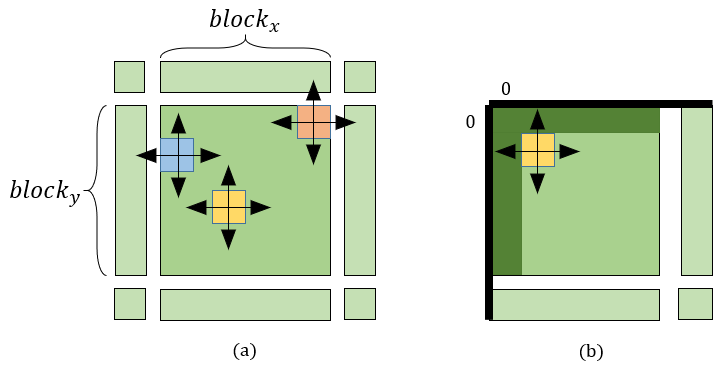
\includegraphics[width=0.9\linewidth]{shmemaccessv3.png}
\caption{Shared Memory with halos. (version 3)}
\label{fig:shmem3}
\end{figure}

Of course, we didn't list as a shared memory implementation version but we could use no shared memory at all too. We will note this as version \textbf{4} in our figures.

\subsection{Cooperative Groups}
Though I did not mention before in this report, I have attempted to use cooperative groups to see how it performs. The main idea behind this was that I could launch a single kernel only, and have the synchronization within the kernel with the cooperative group functions. Also, I would save time from global memory accesses at few points such as sum reduction and standart deviation calculation. For the grid synchronization, we would require a compute capability of 6.0 at least, which only 2 GPUs in KUACC have: \code{GTX\_1080ti} with \code{6.1} and \code{Titan\_V100} with \code{7.0}. Anyways, when I tried to launch it like this, I got problems with the occupancy restrictions. The thing is, grid synchronization also restricts the SM occupancies, and as a result I was unable to test my code. I did not go too deep in this, and instead worked on other optimizations. However, I think it might be possible to run this code using cooperative groups with a smarter and less intensive kernel code.

\section{Performance \& Conclusions} 
We will be looking at 3 different block sizes, all separately and then all together. 
\subsection{Block size 32 by 32}
The results we get from running each version is given in figure \ref{fig:rescomp}.
\begin{figure}[h]
\centering
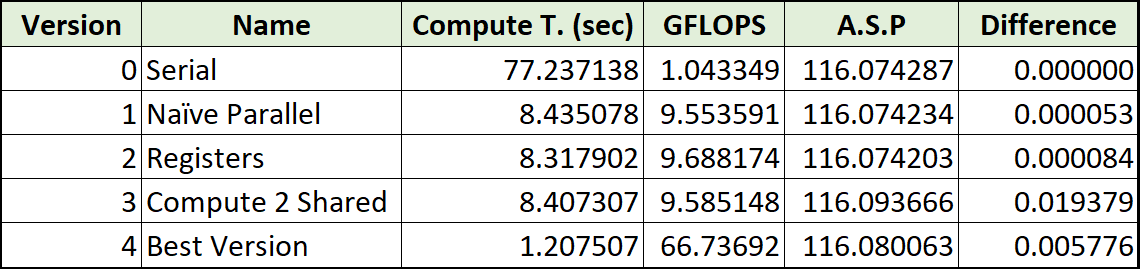
\includegraphics[width=0.9\linewidth]{allresults32.png}
\caption{Comparison of versions on \code{coffee.pgm} with \code{-iter 100} option with $32\times32$ block size. Version is the implementation version, as also specified in the assignment. Compute T. is the compute time output from the program. GFLOPS is the gigaflops output from the program. A.S.P. is the average of sum of pixels output from the program. Difference is the difference between A.S.P. of each program with the serial A.S.P.}
\label{fig:rescomp}
\end{figure}

To determine version 4, we tried all combinations of optimizations, as well as using pinned memory, to choose the best performing one. To reduce the number of combinations (from 16 to 8) we found the best performing shared memory implementation on Compute 1 Kernel, which was v1 (direction-wise halo checking), and used that on compute 2 kernel. That is why we have 4 versions of Compute 1 Kernel but two versions of Compute 2 Kernel, where v1 is direction-wise halo checking and v2 is just global access.

\begin{figure}[h]
\centering
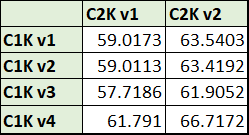
\includegraphics[width=0.45\linewidth]{v4nopin32.png}
\caption{Version 4 combination of kernels without pinned memory, block size $32\times32$. C1K stands for Compute 1 Kernel and it's versions as discussed before. C2K is likewise for Compute 2 Kernel, v1 uses same method as C1K v1 and C2K v2 uses global access only.}
\label{fig:v4nopin}
\end{figure}

\begin{figure}[h]
\centering
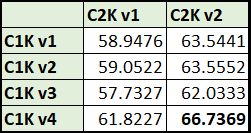
\includegraphics[width=0.45\linewidth]{v4yepin32.png}
\caption{Version 4 combination of kernels with pinned memory, block size $32\times32$. C1K stands for Compute 1 Kernel and it's versions as discussed before. C2K is likewise for Compute 2 Kernel, v1 uses same method as C1K v1 and C2K v2 uses global access only.}
\label{fig:v4yepin}
\end{figure}

From figures \ref{fig:v4nopin} and \ref{fig:v4yepin} we concluded that using C1K v4 and C2K v2 with pinned memory performs best. In other words, we use shared memory sum reduction for the reduction part, however, use global access only for the Compute 1 and Compute 2 kernels. 
Now, we should explain why shared memory performed worse than global access. First let us make an observation, using global access each thread makes 5 accesses. One for the middle and one for each neighbor. So that is $5 \times block_x \times block_y$ accesses. Let us recall the memory access count for direction-wise shared memory: $2 \times block_x + 2 \times block_y + block_x \times block_y$. Considering a $32\times32$ block, we get $5120$ for global access only and $1152$ for the shared memory. However, numbers aside, these happen in parallel and in the case of shared memory threads wait for each other before they begin computation. This is one point of stalling. 
Another point of stalling is during bank conflicts when neighbor threads try to compute on the same index, for example if an index's all 4 neighbors try to use that index at the same time, we get 4 threads attempting access on the same bank, which is a bank conflict.

We also use pinned (page-locked) memory for the image to increase the speed of transferring data from host to device and back. This gave us a slight (0.02 GFLOPs) performance increase as we see in the figures above.

\subsection{Block size 16 by 16}
The results we get from running each version is given in figure \ref{fig:rescomp16}.
\begin{figure}[h]
\centering
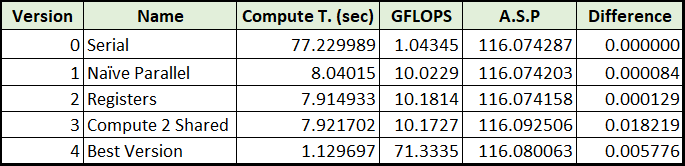
\includegraphics[width=0.9\linewidth]{allresults16.png}
\caption{Comparison of versions on \code{coffee.pgm} with \code{-iter 100} option with $16\times16$ block size. Version is the implementation version, as also specified in the assignment. Compute T. is the compute time output from the program. GFLOPS is the gigaflops output from the program. A.S.P. is the average of sum of pixels output from the program. Difference is the difference between A.S.P. of each program with the serial A.S.P.}
\label{fig:rescomp16}
\end{figure}

We observe similar behaviour as block size $32\times32$. Again, best version uses shared memory sum reduction and global access for both compute kernels as well as pinned memory. Figures \ref{fig:v4nopin16} and \ref{fig:v4yepin16} show the performances of the combination of optimizations.
\begin{figure}[h]
\centering
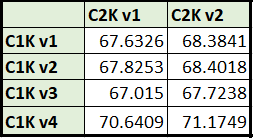
\includegraphics[width=0.45\linewidth]{v4nopin16.png}
\caption{Version 4 combination of kernels without pinned memory, block size $16\times16$. C1K stands for Compute 1 Kernel and it's versions as discussed before. C2K is likewise for Compute 2 Kernel, v1 uses same method as C1K v1 and C2K v2 uses global access only.}
\label{fig:v4nopin16}
\end{figure}

\begin{figure}[h]
\centering
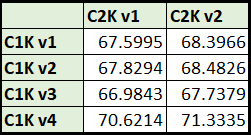
\includegraphics[width=0.45\linewidth]{v4yepin16.png}
\caption{Version 4 combination of kernels with pinned memory, block size $16\times16$. C1K stands for Compute 1 Kernel and it's versions as discussed before. C2K is likewise for Compute 2 Kernel, v1 uses same method as C1K v1 and C2K v2 uses global access only.}
\label{fig:v4yepin16}
\end{figure}

\subsection{Block size 8 by 8}
The results we get from running each version is given in figure \ref{fig:rescomp8}.
\begin{figure}[h]
\centering
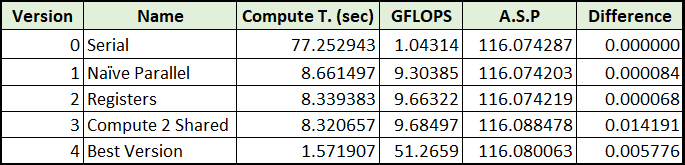
\includegraphics[width=0.9\linewidth]{allresults8.png}
\caption{Comparison of versions on \code{coffee.pgm} with \code{-iter 100} option with $8\times8$ block size. Version is the implementation version, as also specified in the assignment. Compute T. is the compute time output from the program. GFLOPS is the gigaflops output from the program. A.S.P. is the average of sum of pixels output from the program. Difference is the difference between A.S.P. of each program with the serial A.S.P.}
\label{fig:rescomp8}
\end{figure}

This time, though we observe same kind of performance increase over versions, our best version (version 4) is different. When we had $16\times16$ and $32\times32$ block sizes, our best version was when we had global access only for both compute kernels with pinned memory. But when we have block size $8\times8$, we observe that the best version is to have global access for compute 1 kernel, shared memory with direction-wise halo checks for compute 2 kernel and no pinned memory!  Figures \ref{fig:v4nopin8} and \ref{fig:v4yepin8} show the performances of the combination of optimizations.
\begin{figure}[h]
\centering
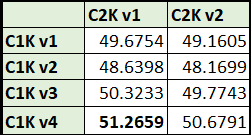
\includegraphics[width=0.45\linewidth]{v4nopin8.png}
\caption{Version 4 combination of kernels without pinned memory, block size $8\times8$. C1K stands for Compute 1 Kernel and it's versions as discussed before. C2K is likewise for Compute 2 Kernel, v1 uses same method as C1K v1 and C2K v2 uses global access only.}
\label{fig:v4nopin8}
\end{figure}

\begin{figure}[h]
\centering
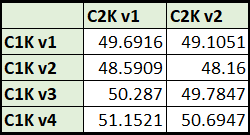
\includegraphics[width=0.45\linewidth]{v4yepin8.png}
\caption{Version 4 combination of kernels with pinned memory, block size $8\times8$. C1K stands for Compute 1 Kernel and it's versions as discussed before. C2K is likewise for Compute 2 Kernel, v1 uses same method as C1K v1 and C2K v2 uses global access only.}
\label{fig:v4yepin8}
\end{figure}

\subsection{Interpreting Differences on Average of Sum of Pixels}
In figures \ref{fig:rescomp}, \ref{fig:rescomp16} and \ref{fig:rescomp8} we might notice that there is a small difference between the serial A.S.P (average of sum of pixels) and other versions's A.S.P.'s. We read images as \code{unsigned char} and convert pixels to \code{float} as we work on them. However, the serial and parallel versions behave on different floating point precisions while they are summing. This is especially evident with the version 4, where we use sum reduction. Version 3 also differs a bit from the serial A.S.P. and we believe the cause is still same. The precision is different and therefore they add up in different ways. For example, when we use compute 2 kernel with shared memory as it is in version 3, and when we use sum reduction and also compute 2 kernel with shared memory, we get different results. However, without the sum reduction the number is more off than when it is implemented. In all three figures \ref{fig:rescomp}, \ref{fig:rescomp16} and \ref{fig:rescomp8} we see this, and though we did not include it here, all combination of optimizations we do with version 4 give the same result: 116.080063.

\subsection{Interpretations of Shared Memory Usage}
\textit{Why did our best version usually prefer global access (and data re-use with registers) instead of shared memory?} We have discussed these before but it is also appropriate to re-state them here as well. 
\begin{itemize}
	\item We may observe 4-way bank conflicts while using shared memory, due to the nature of the algorithm.
	\item The loading phase may stall some of the threads that are waiting to compute in the block.
	\item For the fully shared memory version (version 3), there is an additional redundant transfer of data on halo regions, which may decrease the performance.
\end{itemize}
It is also possible that the resource limits of SM cause stalling. In other words, let us say each thread grabs $r$ registers. This means that for every active block in SM we will have $block_x\times block_y \times r$ memory for registers and $block_x\times block_y$ for shared memory. If SM can not handle this much memory requirement at once, some blocks will be stalled and not all of them will run in parallel. This will cause a drop in performance, and evidently, it did in our case.

\subsection{Interpretations of Block Size}
\textit{Why is block size $16\times16$ faster than $32\times32$ and $8\times8$ block sizes? Also, why does the best version change for $8\times8$ block size?} We used figure \ref{fig:speedallintro} at the start as per request of assignment, but we will use it here again (figure \ref{fig:speedallintro2}) to match the context.
\begin{figure}[h]
\centering
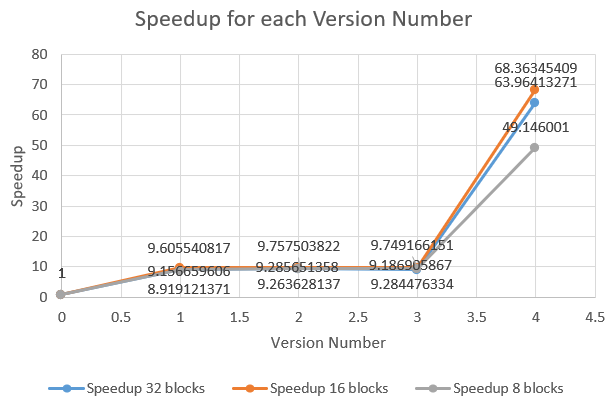
\includegraphics[width=0.92\linewidth]{speedall.png}
\caption{Speedups for each version. Version 0 is serial. The rest are parallel. Version 1 is using global access only. Version 2 is using registers for data re-use. Version 3 uses shared memory on compute 2 kernel. Version 4 is a combination of optimizations and is the best version.}
\label{fig:speedallintro2}
\end{figure}
Recall that we discussed block stalling in the previous subsection, where SM could not handle the required amount of resources thus stalled some blocks. When it comes to smaller blocks, SM could perhaps run more blocks concurrently and therefore achieve greated performance. In other words, we have a finer grained task at our hand. This is what we observe for $16\times16$ block size, however when task is too fine grained, as it is in $8\times8$, we lose performance. This might be relevant to the fact that we load halo regions for each block: the more blocks we have the more halo regions we would have to load. This might be reflecting as a drop in performance.
Regarding the figure, notice that the best versions of $32\times32$ and $16\times16$ block sizes use shared memory only at the sum reduction part. This, however, seems to be affecting the performance greatly, thus putting $16\times16$ block size at the top.

\end{document}